\documentclass[10pt,a4paper,ngerman]{scrartcl}
\usepackage[utf8]{inputenc}
\usepackage[ngerman]{babel}
\usepackage[T1]{fontenc}
\usepackage{amsmath}
\usepackage{amsfonts}
\usepackage{amssymb}
\usepackage{makeidx}
\usepackage{graphicx}
\usepackage{epstopdf}
\usepackage[onehalfspacing]{setspace}
\usepackage{array}
\usepackage{upgreek}
\usepackage{float}
\usepackage{csquotes}
\usepackage{chemformula}
\usepackage{chemgreek}
\usepackage{chemmacros}
\chemsetup{modules=all}
\usepackage{tikz}
\usepackage{siunitx}
\sisetup{locale = DE,per-mode = symbol}
\usepackage{esvect}
\usepackage{geometry}
\usepackage{pdfpages}
\usepackage[font=small]{caption}
%\usepackage[version=4]{mhchem}
\usepackage[backend=biber, style=chem-angew]{biblatex}
\addbibresource{Elektro.bib}
\usepackage{tabularx, booktabs, multirow}
\usepackage[pdfborder={0 0 0}]{hyperref}
\usepackage{scrlayer-scrpage}%Header für die KOMA-script -Klasse
%\usepackage{hyperref}
\usepackage{pgfplots}
\usepackage{textgreek}


\newcommand{\tildenu}{{\fontencoding{LGR}\selectfont\accperispomeni\textnu}}
\captionsetup{format=plain}
\chemsetup[phases]{pos=sub}
\chemsetup[redox]{pos=top}
\chemsetup[redox]{align=center}
%\chemsetup[redox]{explicit-sign=true}
%\chemsetup[redox]{roman=false}
\newcommand{\celsius}{^{\circ}\mathrm{C}}
\parindent0pt
\sloppy
\DeclareChemPhase{\s}{s}
\DeclareChemPhase{\l}{l}
\DeclareChemPhase{\g}{g}
\renewcaptionname{ngerman}{\figurename}{Abb.}
\renewcaptionname{ngerman}{\tablename}{Tab.}
\geometry{bottom=100pt} \geometry{top=80pt}
\newcommand{\m}{\mathrm{m}}
\newcommand{\K}{\mathrm{K}}
\newcommand{\J}{\mathrm{J}}
\newcommand{\gr}{\mathrm{g}}
\newcommand{\kg}{\mathrm{kg}}
\newcommand{\mol}{\mathrm{mol}}
\newcommand{\Pa}{\mathrm{Pa}}
\newcommand{\ad}{\mathrm{ad}}
\newcommand{\de}{\mathrm{de}}
\newcommand{\gmol}{\mathrm{\frac{g}{mol}}}
\newcommand{\JKmol}{\mathrm{\frac{J}{K \cdot mol}}}
\newcommand{\kgmss}{\mathrm{\frac{kg}{m \cdot s^2}}}
\newcommand{\loge}{\mathrm{ln}}


\begin{document}
\begin{titlepage}
	\vspace*{2,5cm}
	\begin{center}
		\begin{LARGE}
			\textbf{Polymer Chemie}\\
			\textbf{Elektropolymerisation}\\
		\end{LARGE}
		\vspace{1cm}
		\textbf{Universität Stuttgart}\\
		\vspace*{1,5cm}
		\begin{tabular}{lp{7,5cm}l}
			Author 1:     &Laurens Viehoff\\
            Author 2:     &Felix Roth\\   
			E-Mail 1:      &st183688@stud.uni-stuttgart.de\\
            E-Mail 2:      &st188157@stud.uni-stuttgart.de  \\
			Student-ID 1: & 3676761   \\ 
            Student-ID 2: & 3711192 \\ \\
			Assistentin:  & Xiuming Sun  \\ \\ 
		\end{tabular}
	\end{center}

    
\end{titlepage}
\thispagestyle{empty}
\renewcommand{\thepage}{\arabic{page}}
\newpage
\tableofcontents
\setcounter{page}{1}
\renewcommand{\thepage}{\arabic{page}}
\newpage

\section{Theorie}

	Damit ein Polymer leitfähig ist, muss eine alternierung zwischen $\pi$ und $\sigma$ Bindung am Polymerrückgrad vorliegen.
	Dies ist vorallem wichtig da durch das konjugierte System der Kohlenstoff in einer sp$^2$ konfiguration vorliegt 
	und somit ein vollständig besetztes $\pi$-Orbital und ein unbesetztes $\pi^*$-Orbital aufweist. 
	Wird das System nun um mehrere Kohlenstoffe erweitert, bilden sich wie in Abbildung \ref{VB_CB} zwei Bereiche, diese werden auch Valenzband (unten) 
	und Leitungsband (oben) genannt.
	
		\begin{figure}[H]
			\centering
			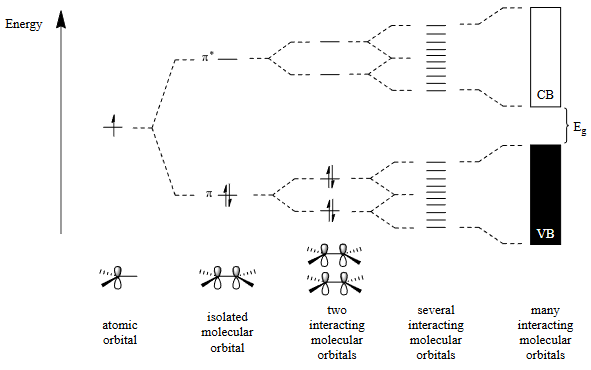
\includegraphics[scale = 0.75]{Bilder/VB-CB.png}
			\caption{Molekül-Orbital-Schema zur Bildung des Valenz- und Leitungsband. \cite{polyskript}}
			\label{VB_CB}
		\end{figure}

	Die Bandlücke $E_\text{g}$ ist dabei der Bereich zwischen den beiden Bändern.
	Je größer diese ist desto schlechter leitet der Stoff, da im Falle von Leitung ein Elektron vom Valenzband in das Leitungsband übergehen muss.
	Dieser Abstand kann durch Oxidation oder Reduktion verkleinert werden. 
	In Abbildung \ref{thiophen} ist dies am Beispiel von Thiophen gezeigt, dabei sind die beiden dotierten Strukturen gezeigt.
	Im laufe der Oxidation werden Elektronen aus dem HOMO entnommen, im falle der Reduktion wird ein elektron in das LUMO aufgenommen.
	Dabei entstehen Ladungen, weshalb dieser Vorgang auch als charging bekannt ist.
	
		\begin{figure}[H]
			\centering
			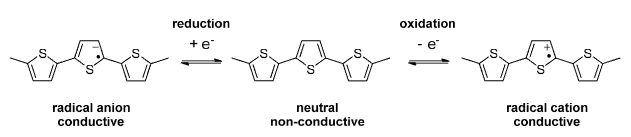
\includegraphics[scale = 0.75]{Bilder/thiophen.png}
			\caption{Oxidation und Reduktion von Thiophen mit Änderung der Elektronischen Struktur. \cite{polyskript}}
			\label{thiophen}
		\end{figure}

	Diese Elektronenabgabe bzw Aufnahme kann auch Einfluss auf die physischen Eigenschaften nehmen, wie zB. die Farbe.
	Diese Materialien werden auch Elektrochrom genannt. So ist Beispielsweise PEDOT im oxidierten Zustand transparent und wird nach reduktion dunkelblau. 
	Dies lässt sich durch verkleinerung der Bandlücke erklären. So ändert sich bei Änderung des elektronischen Zustands auch das Absorptionsspektrum und damit auch die Farbe. 
	Dementsprächend lässt sich eine Verkleinereung der Bandlücke erklären. \\

	Das Redoxverhalten der Stoffe wird bei der Cyclovoltametrie ausgenutzt.
	Hierbei wird im laufe des Experiments ein linearer Potentialdurchlauf mit konstanter Scanrate
	($V$) in einem bestimmten Potentialfenster durchgeführt. Am Ende des Potentialfensters ($E\lambda$)
	wird die Richtung des Durchlaufs umgekehrt und das Potential linear verringert (mit
	derselben Spannung $V$), bis das Startpotential wieder erreicht ist. 
	Während dieses Potentialdurchlaufs wird der Strom aufgezeichnet und gegen das
	angelegte Potential aufgetragen.
	Die Messung selbst wird über ein drei Elektroden Aufbau ermittelt. 
	Dabei ist eine der drei Elektroden die Arbeitselektrode, eine die Gegenelektrode und die dritte die Referenzelektrode.
	Diese Elektroden werden dabei in eine Lösung mit der zu Untersuchen Substanz gegeben.
	Die Referenzelektrode hat dabei den Nutzen das Potential zu kontrollieren und um den Start des Potentials festzulegen.
	Dabei werden meist Standard Wasserstoff Elektroden (SHE) oder Silber/Silberchlord Elektroden verwendet.
	Im Falle von organischen Lösungsmitteln wird ein Ferrocen/Ferrocenium zusatz verwendet, da die vorher genannten Elektrode nur in Wasser ein 
	gleichbleibendes Potenzial besitzt. Ebenfalls muss das Potenzial des Ferrocen/Ferrocenium Redoxpaars vorerst gemessen werden, da diese je nach 
	erhalt der Elektrode ein anderes Potential aufweist.
	%Frage 5 fertig beantworten
	Ein Potentiometer stellt dabei das Potential zwische Referenzelektrode- und Gegenelektrode ein, sodass der Potentialunterschied $\Delta E$ dem eingestellten Wert entspricht.

		\begin{figure}[H]
			\centering
			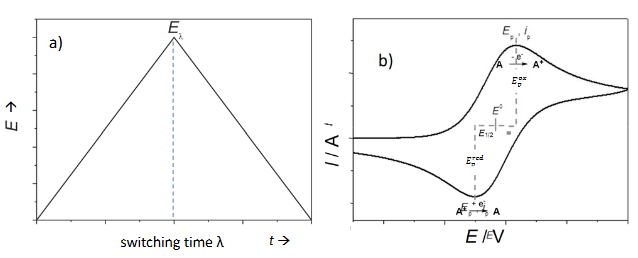
\includegraphics[scale = 0.75]{Bilder/DiagrammeCV.png}
			\caption{Die Abbildung zeigt einmal die Spannungskurve (links) und die dazugehörige Stromstärke (rechts), die bei der angelegten Spannung $V$ detektiert wird. \cite{polyskript}}
			\label{CV-Diagramme}
		\end{figure}

	
\section{Durchführung}

	Der Versuch wurde unter Stickstoffatmosphäre durchgeführt. Als Elektroden wurde eine Platin-Platte als Gegenelektrode verwendet, 
	ein Ferrocen/Ferrocenium Zusatz wurde verwendet und 
	als Arbeitselektrode wurde eine mit Glas überzogene ITO (Indium-Zinn-Oxid) Elektrode verwendet.
	Als Elektrolytlösung wurden \SI{6}{ml} einer 0.1 M \ch{NBu4PF6/MeCN}-Losung verwendet. 
	Für die Polymerisierung wurde zu der Elektrolytlösung EDOT hinzugegeben, sodass dessen Konzentration $c = \SI{0,2}{M}$ war.
	Dann wurde eine Spannung von $\SI{-0,4}{V}$ angelegt und mit einer Potentialvorschubsgeschwindigkeit von $\SI{20}{\frac{mV}{s}}$ auf 
	$\SI{1,5}{V}$ erhöht, bevor es dann wieder mit der selben Potentialvorschubsgeschwindigkeit auf $\SI{-1,0}{V}$ herabgesenkt wurde. Dieses 
	Vorgehen wurde dreimal durchgeführt. \\
	Für die Lage des HOMOs von P3HT wurde von keiner Spannung und einer Potentialvorschubsgeschwindigkeit von $\SI{20}{\frac{mV}{s}}$ auf 
	$\SI{1,2}{V}$ erhöht und anschließend auf $\SI{-0,3}{V}$ herabgesenkt. Das wurde erneut dreimal durchgeführt. Für die Lage des LUMOs von 
	P3HT wurde das gleiche Vorgehen verwendet, aber die maximale Spannung lag bei $\SI{0,4}{V}$ und die minimale bei $\SI{-2,1}{V}$.\\
	Die Untersuchung der Elektrochromie von PEDOT wurde über alternierung der Potentiale $\SI{1,0}{V}$ und $\SI{-1,0}{V}$ durchgeführt. Die 
	Die Zeit für die die Potentiale jeweils angelegt waren, waren $\SI{3}{s}$, $\SI{0,5}{s}$ und $\SI{0,3}{s}$.\\
	Zum Schluss wurde zur Skallierung noch das Potential der Ferrocen/Ferrocenium Elektrode bestimmt, bei welcher die Potentialvorschubsgeschwindigkeit 
	gleich blieb, aber die maximale Spannung bei $\SI{0,7}{V}$, die minimale Spannung bei $\SI{-0,2}{V}$ lag und die Zyklen fünfmal wiederholt 
	wurden. Bei diesem Versuchsteil wurde ebenfalls die \ch{Ag/Ag^+}-Elektrode als Referenzelektrode gewählt und als Arbeitselektrode wurde eine 
	Gold-Elektrode verwendet.
	
\section{Auswertung}

	\subsection{Standardmessung der Ferrocen/Ferrocenium Redoxpaar}

		Das elektrische Potential kann nicht vollständig abgegeben werden, weswegen innerhalb des ersten Versuchsteil ein Standardpotential festgelegt wurde.
		Dabei wurde ein Ferrocen/Ferrocenium (Fc/Fc$^+$) Redoxpaar verwendet mit einer Ag/AgCl-Elektrode als Gegenelektrode.
		Das aufgenommene CV ist in Abbildung \ref{CV-Fe} aufgezeigt.
			\begin{figure}[H]
				\centering
				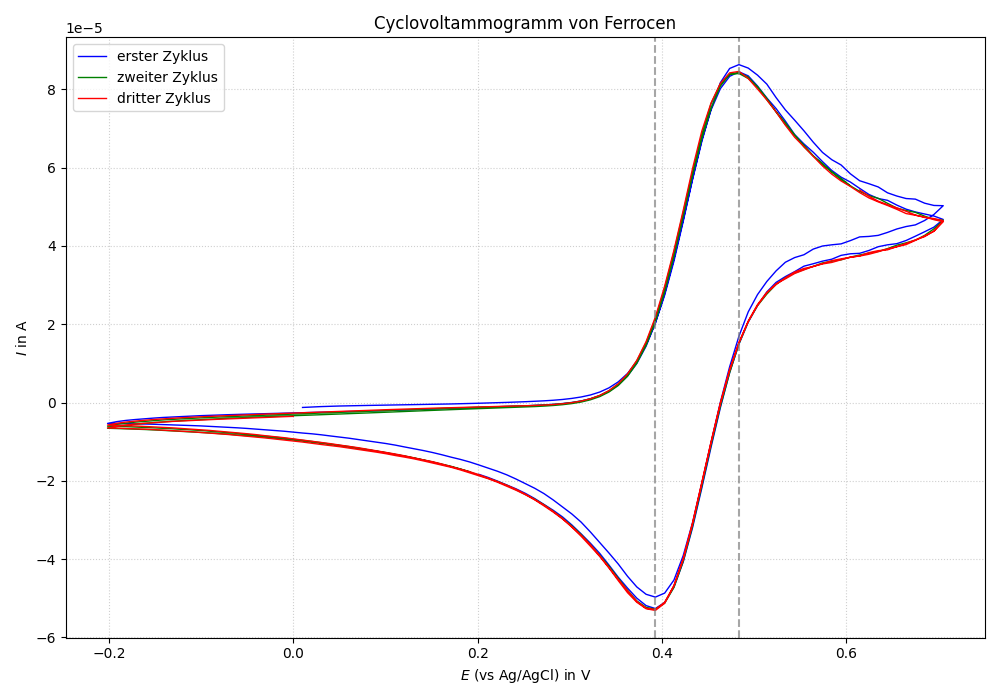
\includegraphics[scale = 0.5]{Bilder/Ferrocen.png}
				\caption{Die Abbildung zeigt das CV von einem Ferrocen/Ferrocenium Redoxpaar mit einer Pt-Elektrode als Gegenelektrode.
				Die gestrichelten Linien sind dabei $E_\text{max}, E_\text{min}$.}
				\label{CV-Fe}
			\end{figure}

		Die gestrichelten Linien markieren dabei das Minimum sowie das Maximum welche das Ox.- bzw Red.-Potential darstellen.
		werden diese beiden Werte gemittelt, erhält man den $E_{1/2}$ Wert. Welcher das Standardpotential der Elektrode darstellt und in den 
		folgenden Versuchen benötigt wird.
		Der Mittelwert der sich bei diesen Werten bildete, lag bei

			\begin{eqnarray*}
				E_{1/2} =& \frac{E_\text{max} + E_\text{min}}{2}\\
				=& \frac{\SI{0,483}{V} + \SI{0,393}{V}}{2} \\
				=& \SI{0,438}{V} \text{.}
			\end{eqnarray*}

			
	\subsection{Elektropolymerisation von EDOT}	

		Der folgende Graph \ref{EDOT} zeigt das CV-Diagramm der Polymerisation von EDOT.
		Durch analysieren des Graphen werden nicht nur die drei Oxidationspeaks rechts erkennbar, sondern auch ein kleiner Peak im Bereich von $\SI{-1,1}{V}$ - $\SI{0,6}{V}$ zu erkennen.
		Welcher vorallem im dritten zyklus deutlich wird.
		Dieser lässt sich durch bereits vorhandenes PEDOT erklären welches oxidiert wird. 
		Dabei ist wichtig, dass PEDOT ein geringeres Oxidationspotential hat und daher leicht oxidiert werden kann.  
			
			\begin{figure}[H]
				\centering
				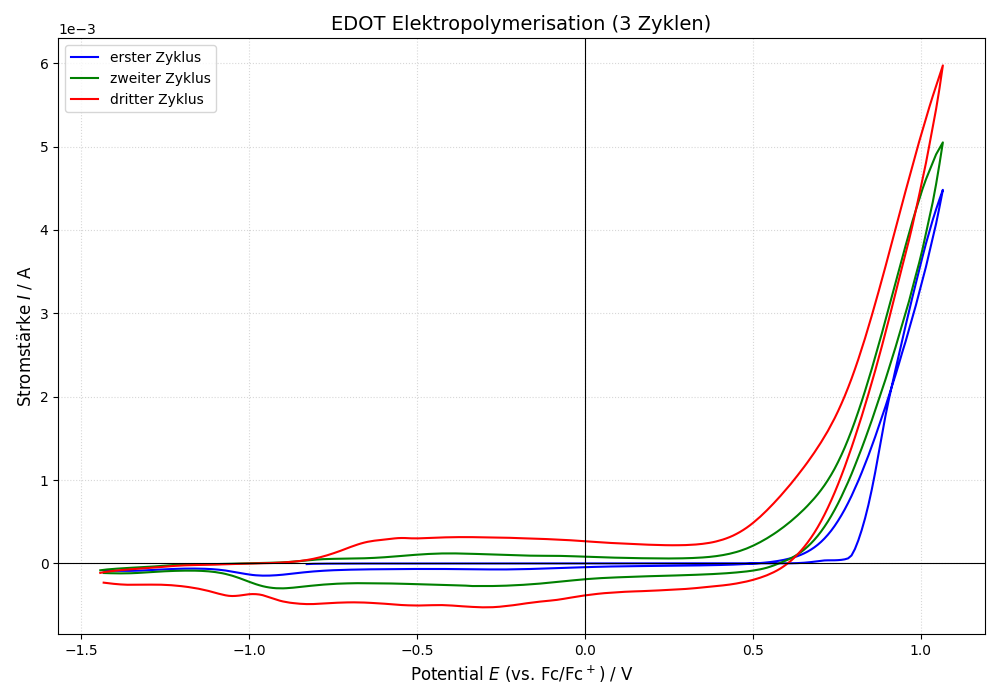
\includegraphics[scale = 0.5]{Bilder/EDOT.png}
				\caption{Zu erkennen ist das CV-Diagramm, welches das Oxidationsverhalten während der Elektropolymerisation von EDOT zeigt.}
				\label{EDOT}
			\end{figure}
\newpage
		In der folgenden Abbildung \ref{EDOT-Mechanismus} ist der Mechanismus dieser PEDOT Polymerisation aufgezeigt. 
		Bei diesem findet eine Bildung eines Radikals statt welches, in diesem Fall, mit einer identischen spezies Rekombiniert.
		Anschließend findet eine Abgabe von Protonen statt, welche eine Rearomatisierung zufolge hat.

			\begin{figure}[H]
				\centering
				
\includegraphics[width = \textwidth]{chemDraw/EDOT.png}
				\caption{Die Abbildung zeigt den Mechanismus der Polymerisation von EDOT zu PEDOT.}
				\label{EDOT-Mechanismus}
			\end{figure}
		

	\subsection{Bestimmung der HOMO- und LUMO-Niveaus}

		Ziel war es hier die energetische Bandlücke zwischen dem HOMO und LUMO zu bestimmen.
		Dafür wurden zunächst die jeweiligen Onset-Potentiale benötigt, welche über die Cyclovoltametrie bestimmt wurden.
		Diese CV-Diagramme sind in Abbildung \ref{CV-P3HT} zu sehen, dabei ist die Oxidation oben und die Reduktion unten.
		Jeweils darüber lässt sich die Energie des HOMO (Oxidation) und die des LUMO (Reduktion) bestimmen. 
		Wichtig anzumerken ist, dass bei Polymeren keine Halbwertspotentiale bestimmt werden können, da diese keine expliziten Kettenlängen besitzen. 
		Denn bei längeren koordinierten $\pi$-Systemen ist der HOMO-LUMO-Abstand kleiner und kann leichter oxidiert oder reduziert werden kann. Daher wird das 
		Onset-Potential bestimmt, welches die mindest Spannung beschreibt, die aufzuwenden ist um das Polymer zu oxidieren/reduzieren.

		
			\begin{figure}[H]
				\centering
				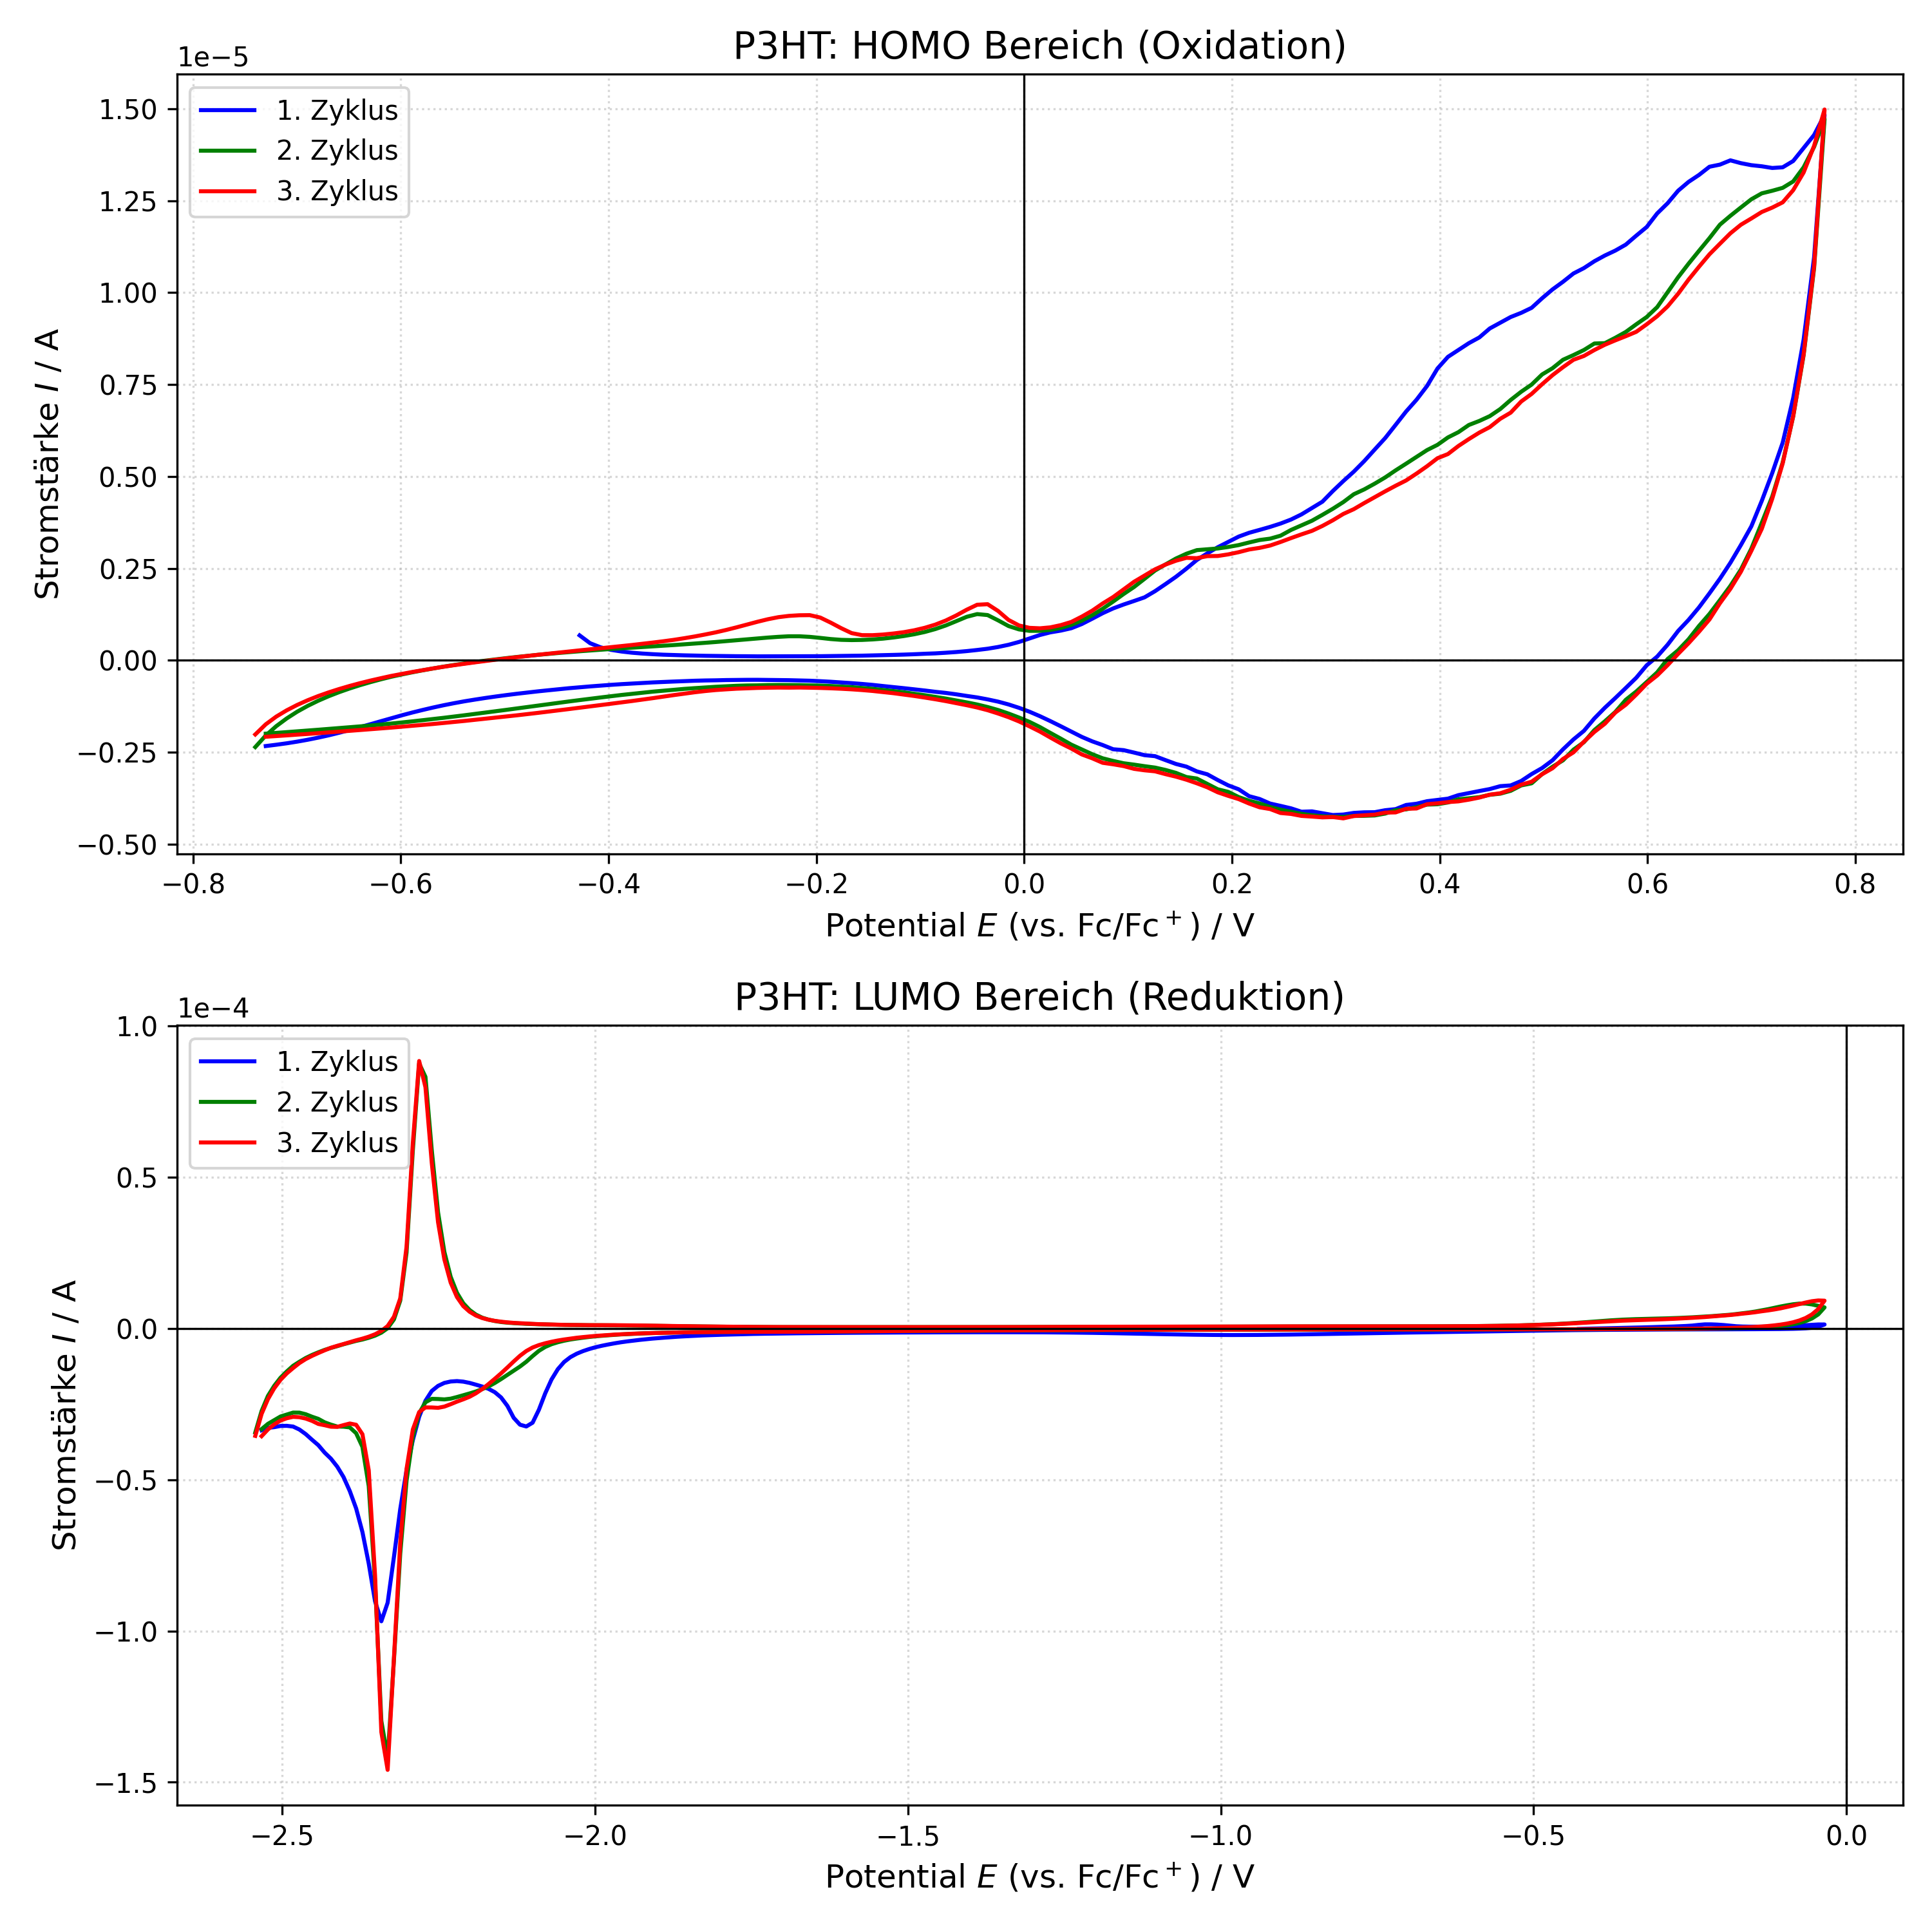
\includegraphics[scale = 0.5]{Bilder/P3HT_HOMO_LUMO_Separate.png}
				\caption{Zu erkennen sind CV-Diagramme von P3HT, der Reduktion (unten) und Oxidation (oben) für jeweils drei Zyklen.}
				\label{CV-P3HT}
			\end{figure}

		Zur Bestimmung der Onset-Potentiale wird einmal die Baseline verlängert und eine Tangente an den Wendepunkt des ersten Signals gelegt. Dieses 
		Vorgehen ist in Abbildung \ref{CV-P3HT-HOMOLUMO} zu erkennen.

			\begin{figure}[H]
				\centering
				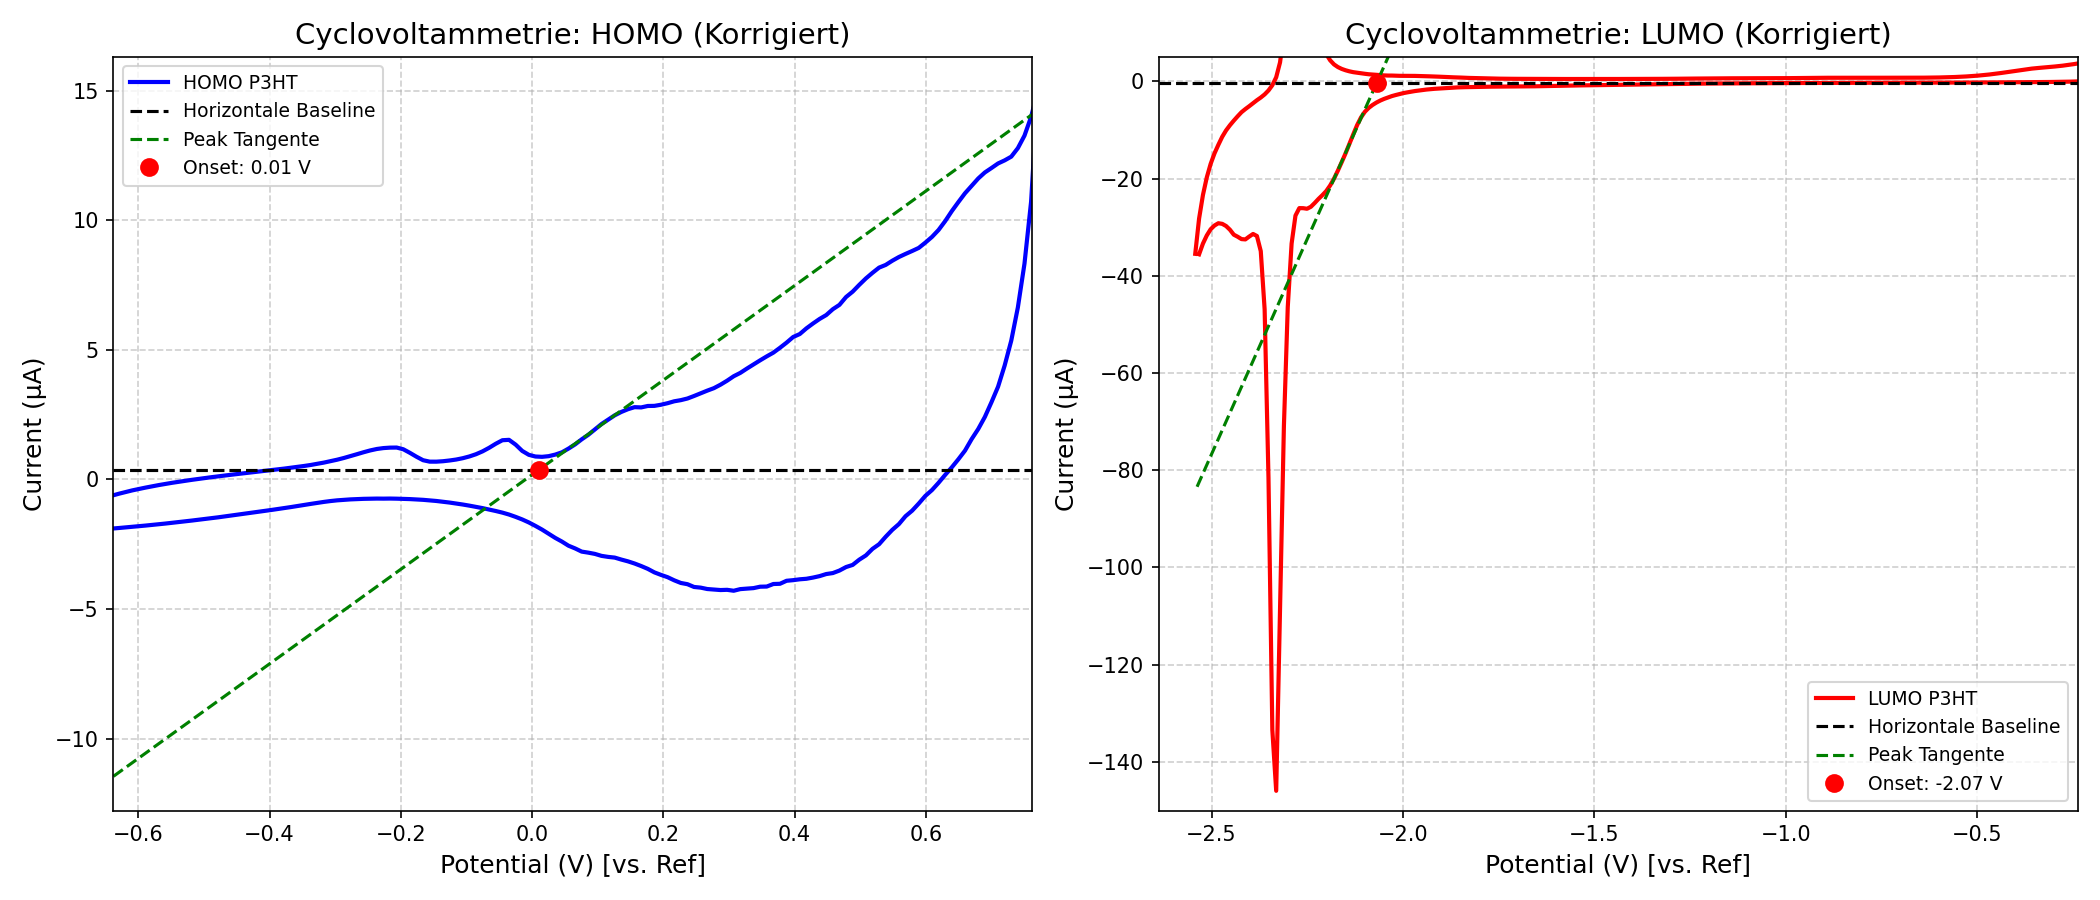
\includegraphics[width = \textwidth ]{Bilder/P3HT_Tangents.png}
				\caption{Zu erkennen sind die Tangenten zur ermittlung des HOMO und LUMO niveaus von P3HT. Ermittelt wurde diese aus dem dritten Oxidations- und Reduktionszyklus.}
				\label{CV-P3HT-HOMOLUMO}
			\end{figure}

		Nach dieser Methode ergab sich ein Oxidations-Onset-Potential von P3HT von $\SI{0,12}{V}$ und ein Reduktions-Onset-Potential von $\SI{-1,63}{V}$. 
		Da das Potential der Fc/Fc$^+$ Elektrode schon in der Achse verrechnet wurde, beschreibt das Onset-Potential der Oxidation die energetische 
		Lage des HOMOs mit $\SI{-0,12}{eV}$ und das Onset-Potential der Reduktion die energetische Lage des LUMOs mit $\SI{1,63}{eV}$. Die 
		Energiedifferenz dieser beiden Werte liegt dabei bei 

		\begin{equation*}
			band \, gap = |\SI{-0,12}{eV} - \SI{1,63}{eV}| = \SI{1,75}{eV}
		\end{equation*}

		und beschreibt den HOMO-LUMO-Abstand.

	\subsection{Elektrochrome Eigenschaften von PEDOT}

		Die folgenden drei Abbildungen zeigen die Stromstäke aufgetragen auf die Zeit für die unterschiedlichen Umkehrzeitintervalle der Untersuchung der
		Elektrochromie des PEDOTs.
		Es konnte bei allen drei ein Farbwechsel festgestellt werden.
		Die Spanne der unterschiedlichen Verfärbungen waren immer ähnlich lang wie die des Intervalls.
		Es wird unteranderem deutlich, dass bei verlängern des Intervalls die Stromstärke eher wieder auf die $\SI{0}{A}$ absinkt. 
		Was durch eine vollständigere Reduktion des PEDOT erklärt werden kann.
		So wird bei der Messung von \SI{0.3}{s} und \SI{0.5}{s} (Abbildung \ref{0.3} und Abbildung \ref{0.5}) schon vor dem erreichen von $\SI{0}{A}$ Umgepolt.

			
			\begin{figure}[H]
				\centering
				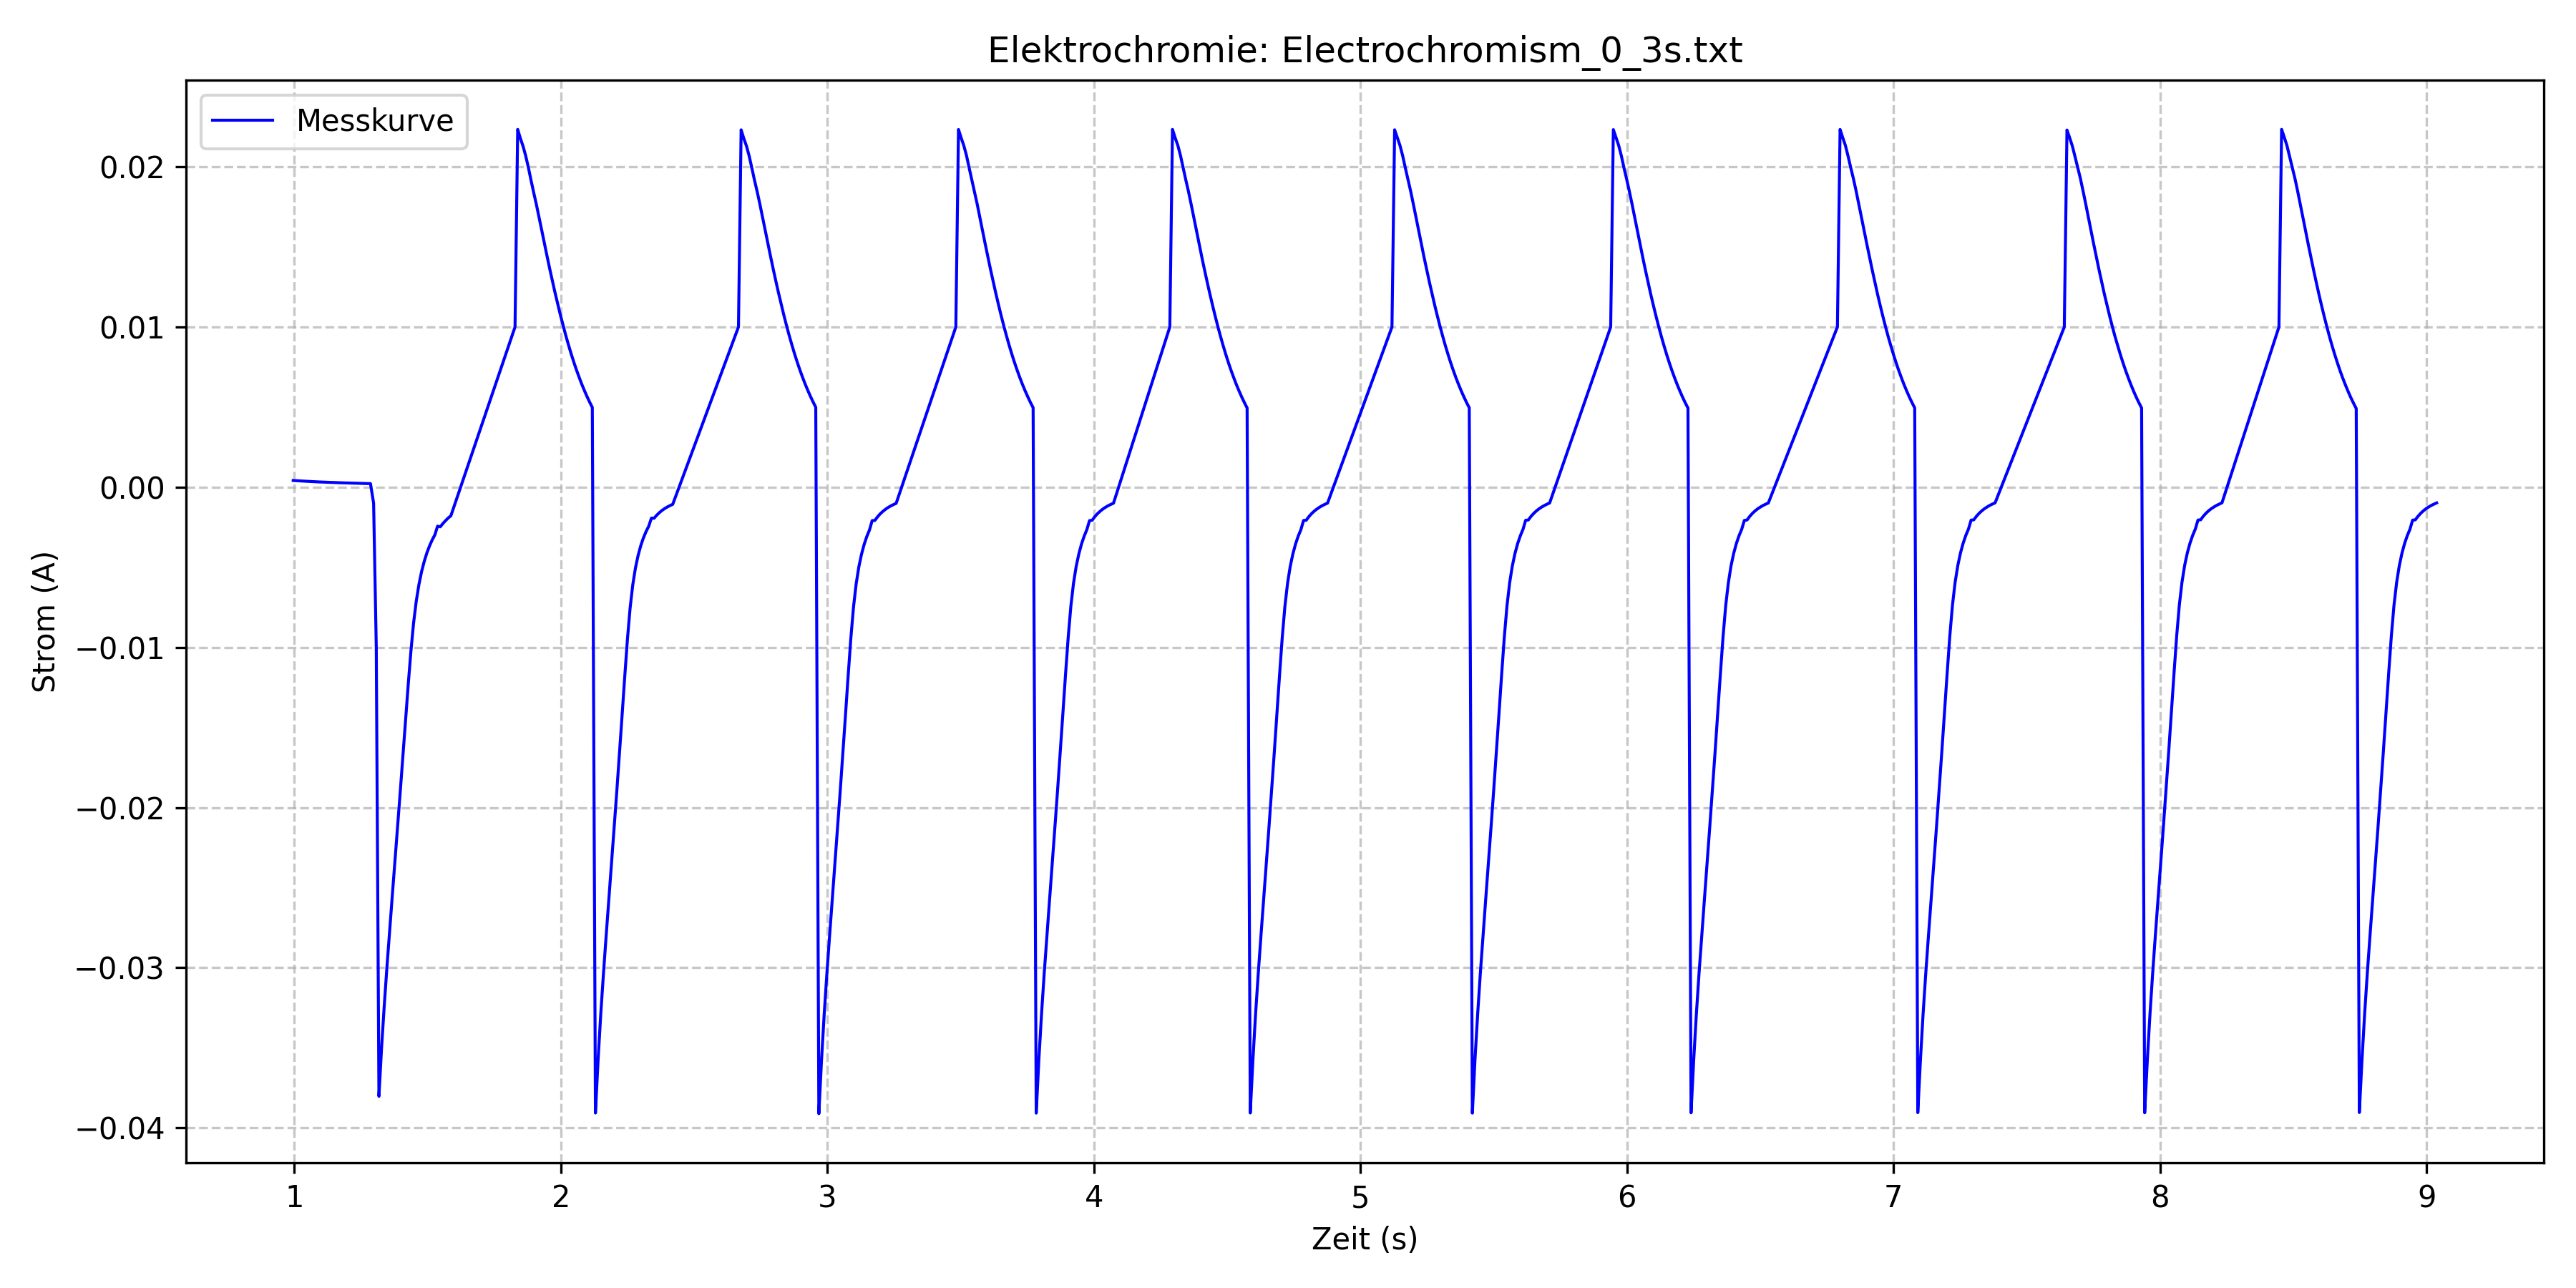
\includegraphics[scale = 0.5]{Bilder/Electrochromism_0_3s.png}
				\caption{Die Abbildung zeigt die zeitlich veränderliche Stromstärke von PEDOT mit einer Spannungsänderungsfrequenz von \SI{0,3}{s}.}
				\label{0.3}
			\end{figure}

			\begin{figure}[H]
				\centering
				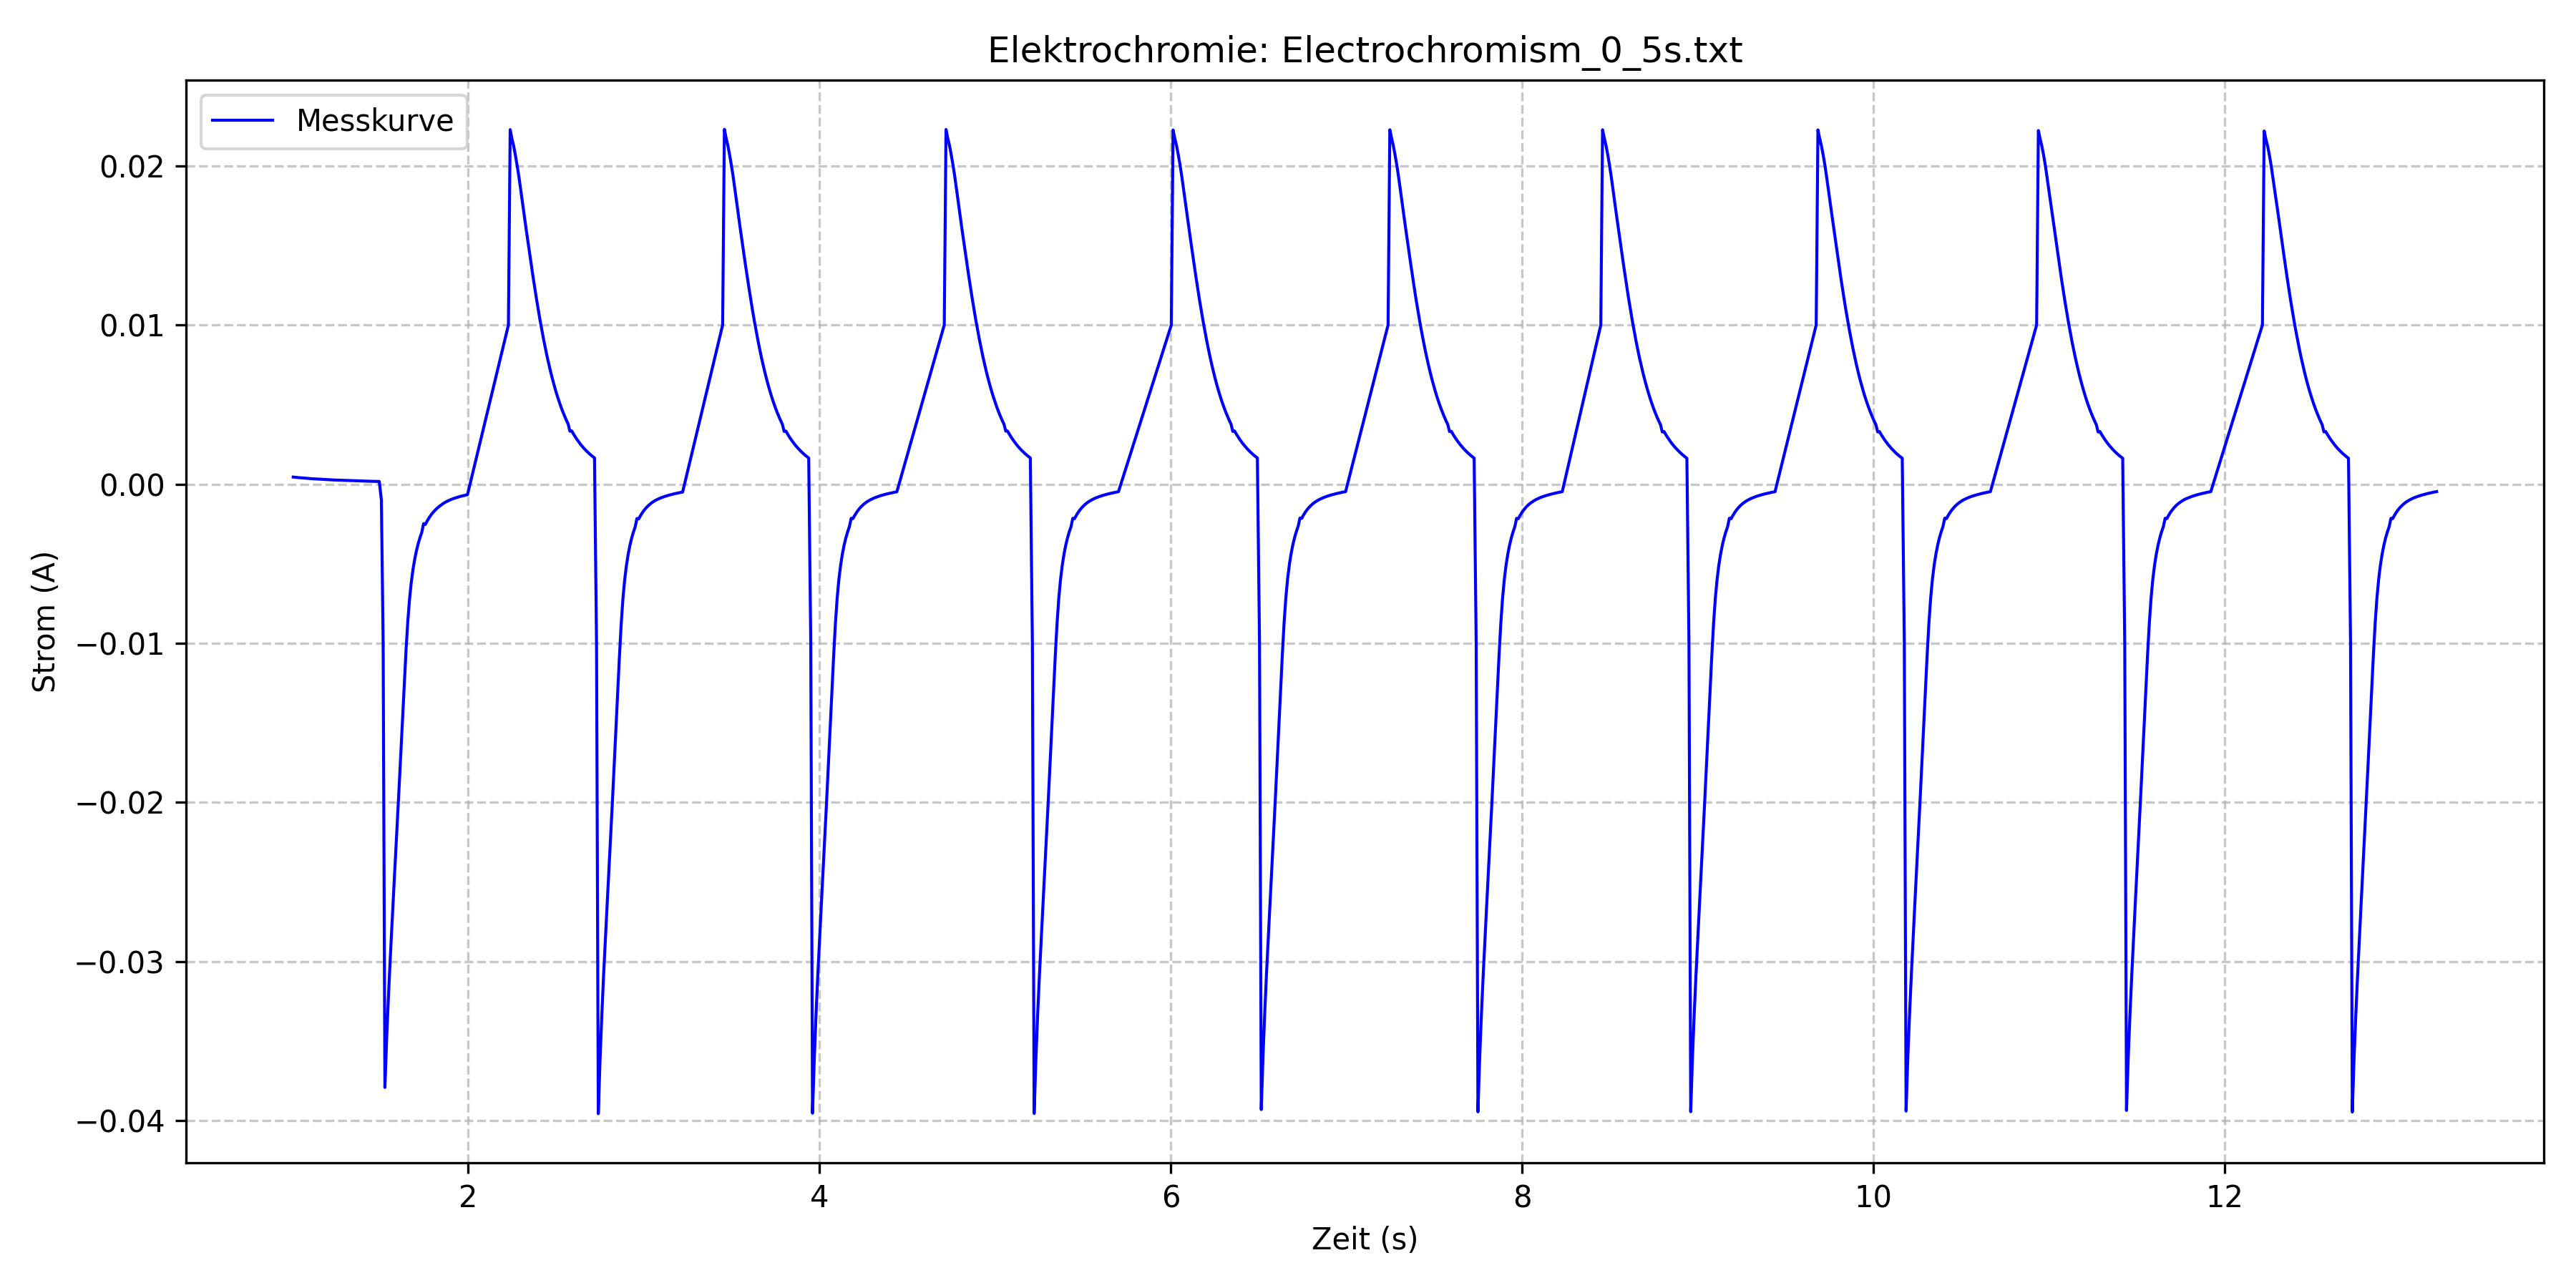
\includegraphics[scale = 0.5]{Bilder/Electrochromism_0_5s.png}
				\caption{Die Abbildung zeigt die zeitlich veränderliche Stromstärke von PEDOT mit einer Spannungsänderungsfrequenz von \SI{0,5}{s}.}
				\label{0.5}
			\end{figure}

			\begin{figure}[H]
				\centering
				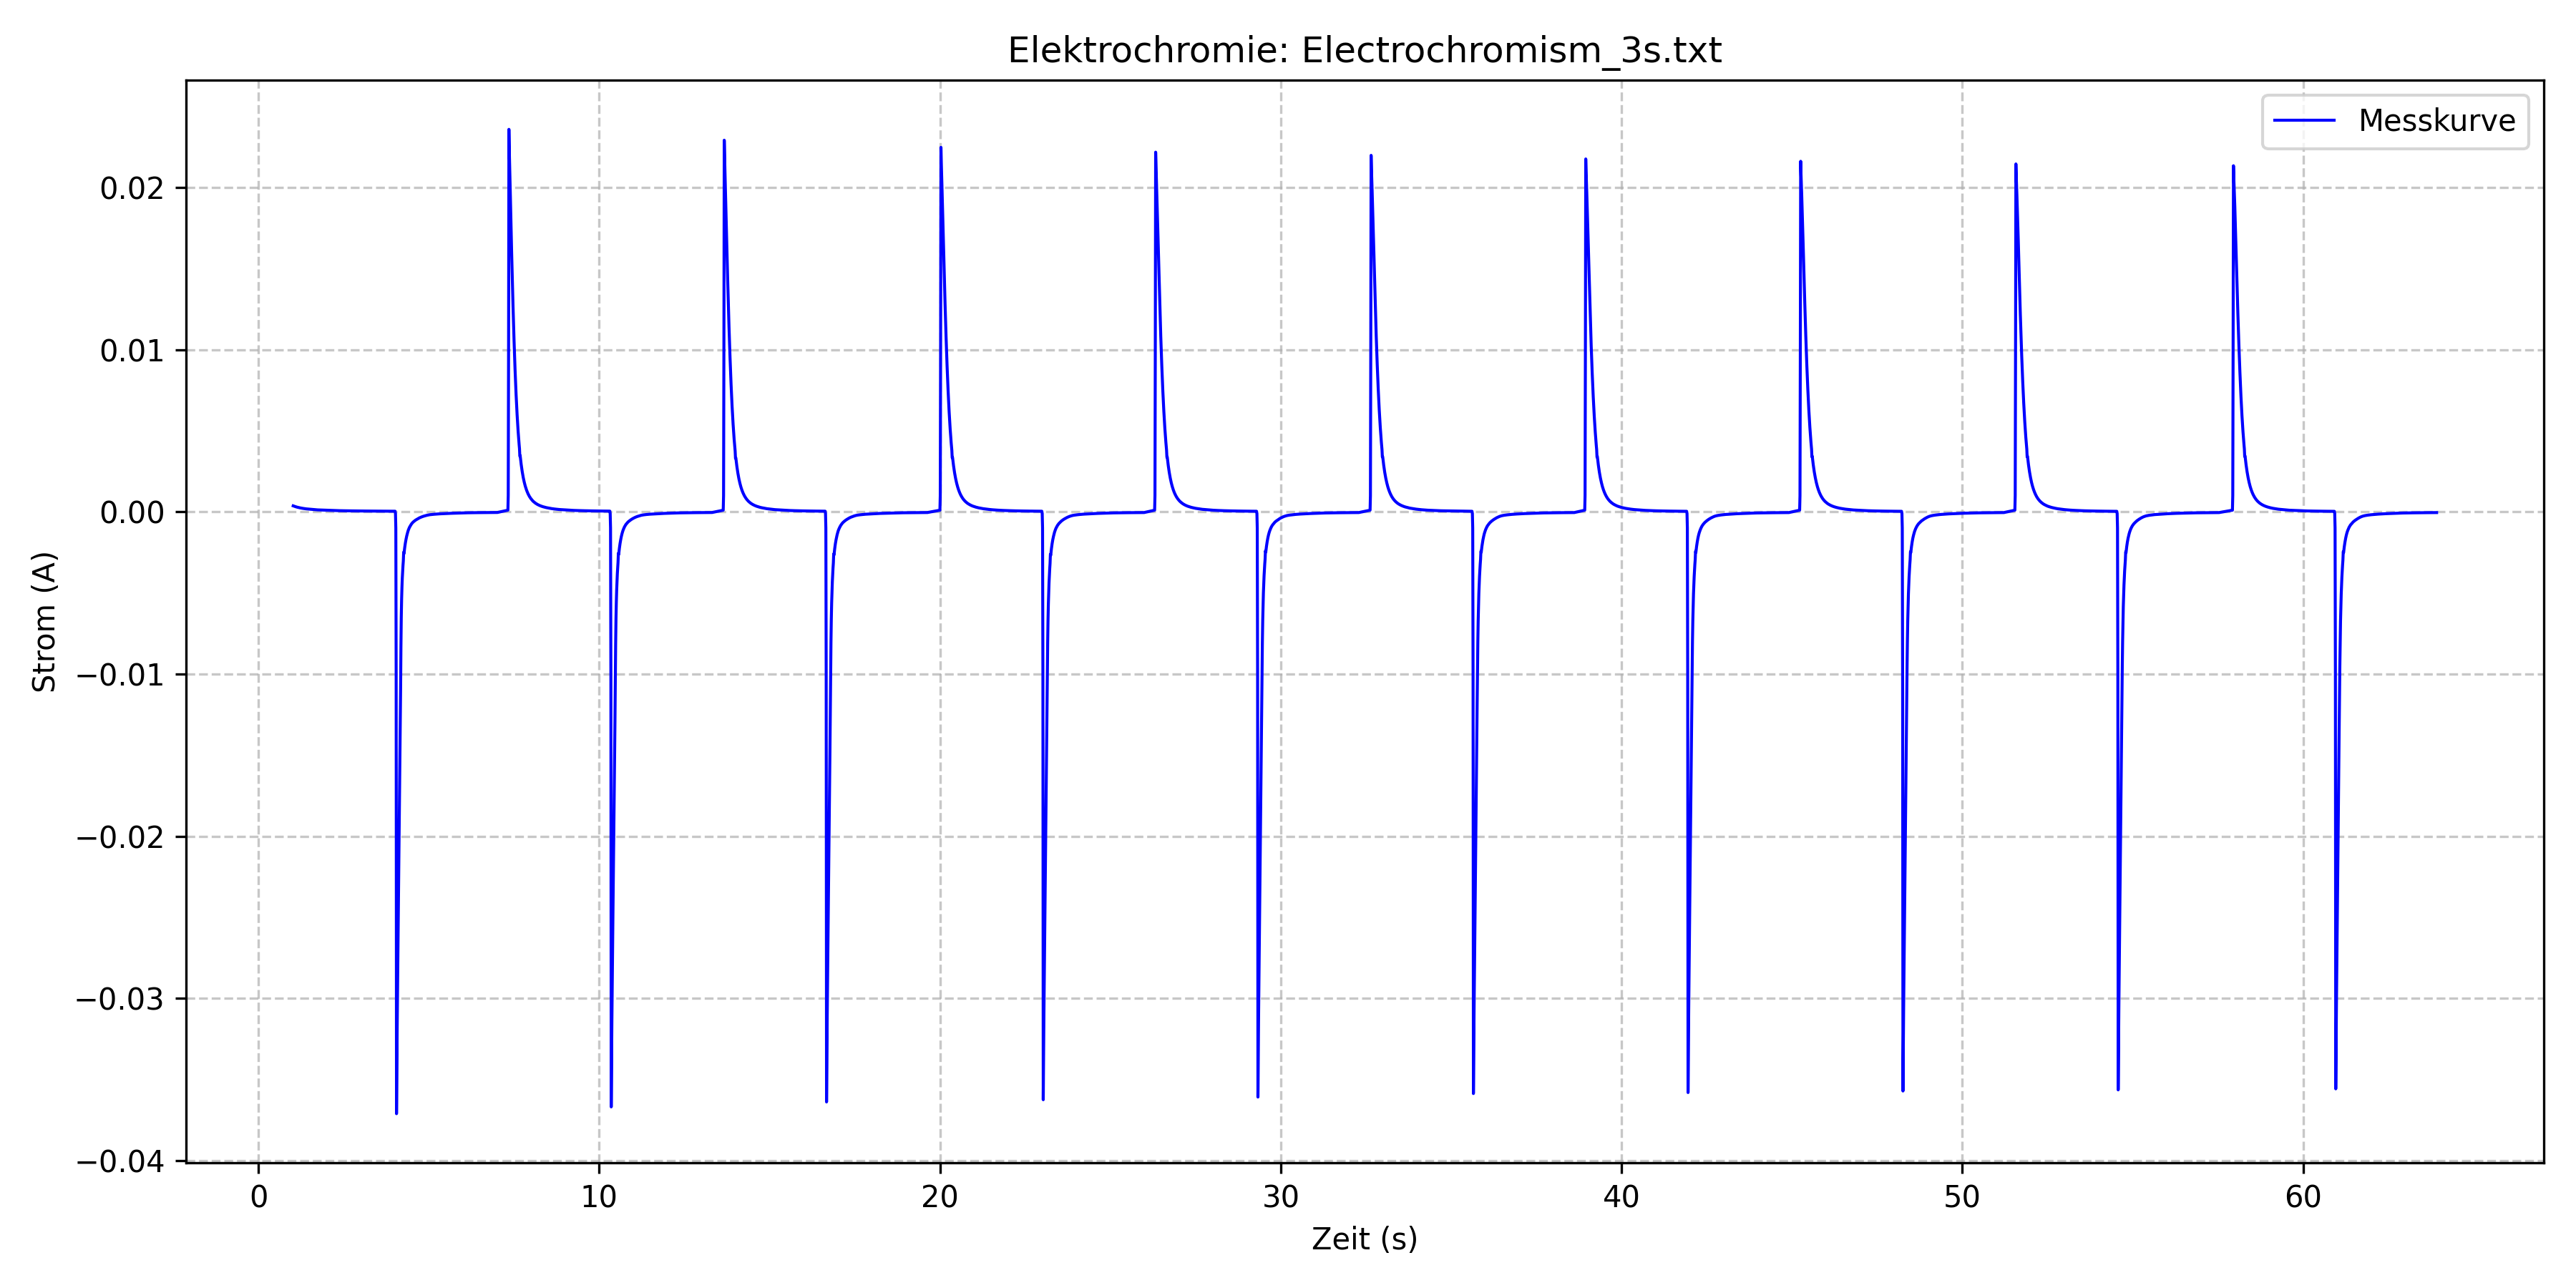
\includegraphics[scale = 0.5]{Bilder/Electrochromism_3s.png}
				\caption{Die Abbildung zeigt die zeitlich veränderliche Stromstärke von PEDOT mit einer Spannungsänderungsfrequenz von \SI{3}{s}.}
				\label{3}
			\end{figure}

\section{Fragen}

		\subsection{Frage 1}

			\begin{figure}[H]
				\centering
				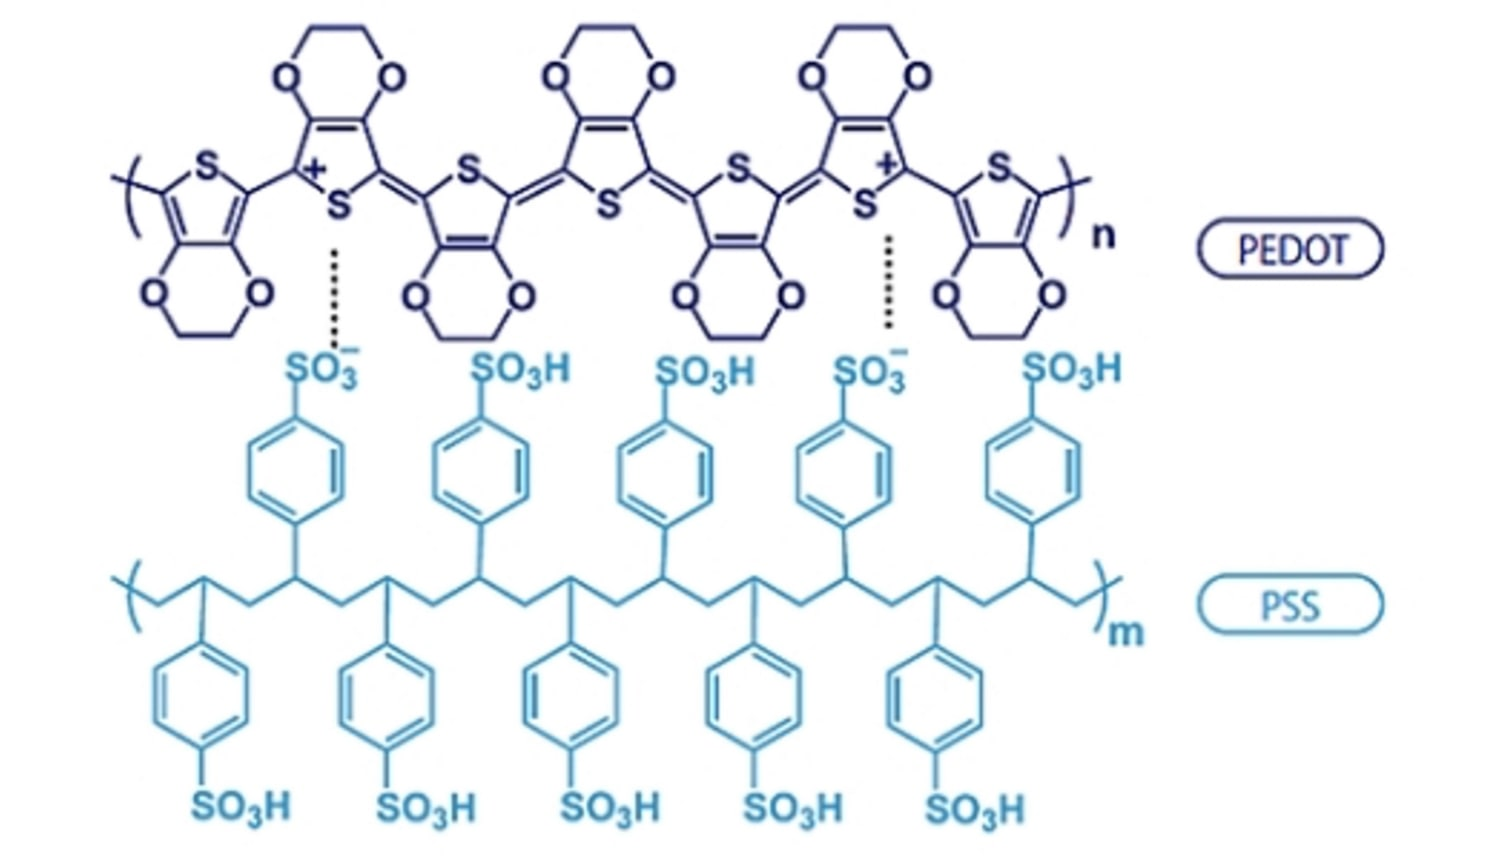
\includegraphics[scale = 0.25]{Bilder/PEDOT-PSS.jpg}
				\caption{Das Bild zeigt die Struktur von PEDOT:PSS. \cite{noauthor_conductive_nodate}}
				\label{PEDOT:PSS}
			\end{figure}

			PEDOT:PSS findet Anwendung in Bildschirmen, Antistatikfilmen, Photovoltaik und Sensoren. \cite{noauthor_conductive_nodate}

		\subsection{Frage 2}

			Im Bild oben zu sehen ist PEDOT und unten das dazugehörige PSS dabei wird das PPS auf das PEDOT dotiert.
			Dabei entsteht eine ionische Bindung zwischen den zwei Ketten. 

		\subsection{Frage 3}

			\begin{figure}[H]
				\centering
				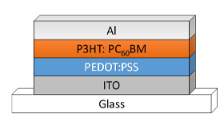
\includegraphics{Bilder/Solarzelle.png}
				\caption{Das Bild zeigt den strukturellen Aufbau einer organischen P3HT:PCBM basierten Solarzelle. \cite{alam_p3htpcbm_2022}}
				\label{Solarzelle}
			\end{figure}

			\begin{figure}[H]
				\centering
				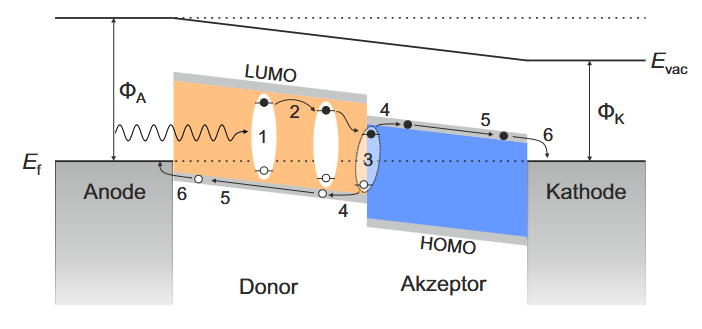
\includegraphics[scale = 0.5]{Bilder/Energiediagramm.png}
				\caption{Das Bild zeigt das Energiediagramm bzw den Ladungstransfer zwischen Donor und Akzeptormaterialeiner organischen Solarzelle. \cite{gruber_analyse_nodate} }
			\end{figure}

\printbibliography
\end{document}